\documentclass[deutsch]{llncs}
\usepackage{url}
\usepackage{graphicx}
\usepackage{listings}
\usepackage{verbatim}
\usepackage{listings}
\lstset{numberbychapter=false}
\usepackage[lined,linesnumbered,german]{algorithm2e}
\SetAlCapFnt{\small}
\SetAlCapNameFnt{\small}
\usepackage{tikz}
\usetikzlibrary{arrows,automata}
\usepackage{xspace}

% for german seminar theses
\usepackage[utf8]{inputenc}
\usepackage[ngerman]{babel}
\usepackage{csquotes}
\usepackage[abbreviate=false,maxbibnames=99,backend=bibtex]{biblatex}
\bibliography{referenzen}

\usepackage{hyperref}

\setcounter{secnumdepth}{2}
\setcounter{tocdepth}{3}

% define custom macros for specific formats or names
\newcommand{\uml}[1]{\texttt{#1}\xspace}
\newcommand{\cd}{\textsf{Klassendiagramm}\xspace}

% Numeriere 3 Ebenen tief (bis subsection)
\setcounter{secnumdepth}{2}

% make a proper TOC despite llncs
\setcounter{tocdepth}{2}
\makeatletter
\renewcommand*\l@author[2]{}
\renewcommand*\l@title[2]{}
\makeatletter

\begin{document}
\def\abstractname{Kurzfassung.}

\pagestyle{plain}
\pagenumbering{roman}

\title{Virtuelle und erweiterte Realität\thanks{Diese Arbeit wurde im Rahmen der LVA ``Wissenschaftliches Arbeiten'' (188.925) im WS18 erstellt.}}


%&&&&&&&&&&&&&&&&&&&&&&&&&&&&&&&&&&&&&&&&&&&&&&&&&&&&&&&&&&&&&&&&&&&&&&&&
% Name and address of the author
%&&&&&&&&&&&&&&&&&&&&&&&&&&&&&&&&&&&&&&&&&&&&&&&&&&&&&&&&&&&&&&&&&&&&&&&&
%\author{Max Mustermann}

%\institute{Technische Universität Wien\\ Bachelorstudium Wirtschaftsinformatik\\ \email{max.mustermann@tuwien.ac.at} \\ Matrikelnr.: 0123456}

%&&&&&&&&&&&&&&&&&&&&&&&&&&&&&&&&&&&&&&&&&&&&&&&&&&&&&&&&&&&&&&&&&&&&&&&&
% Example for more than one authors
%&&&&&&&&&&&&&&&&&&&&&&&&&&&&&&&&&&&&&&&&&&&&&&&&&&&&&&&&&&&&&&&&&&&&&&&&
\author{Barbara Elias\inst{1} \and Yi Wang\inst{2}}

\institute{Technische Universität Wien\\ Bachelorstudium Medizinische Informatik\\ \email{e1028094@student.tuwien.ac.at} \\ Matrikelnr.: 01028094
\and
Technische Universität Wien\\ Bachelorstudium Wirtschaftsinformatik\\ \email{e1633407@student.tuwien.ac.at} \\ Matrikelnr.: 01633407}

\maketitle

% reset footnote counter in case of multiple authors
\setcounter{footnote}{0}

\begin{abstract}
Diese Arbeit beschäftigt sich mit dem Thema virtuelle und erweiterte Realität insbesondere zu Ausbildungszwecken. Im Speziellen werden Publikationen von Mag. Dr. Hannes Kaufmann zur näheren Erarbeitung der Nutzung erweiterter Realität im Hinblick auf den Geometrieunterricht herangezogen. Seine Arbeiten zielen darauf ab, Geometrie begreifbarer zu machen, als es mit der Konstruktion mit Papier und Bleistift möglich ist. Basierend auf schon vorhandener Geometriesoftware wurden VR-Anwendungen konstruiert, die Mathematik verständlicher machen sollen. Die Idee dabei ist, den Schülerinnen und Schülern die Möglichkeit zu geben, mittels VR-Brille um dreidimensionale Objekte zu gehen und diese von neuen, ungeahnten Perspektiven erkennen zu können und damit ein besseres Verständnis für räumliche Geometrie zu bekommen.
\end{abstract}

%&&&&&&&&&&&&&&&&&&&&&&&&&&&&&&&&&&&&&&&&&&&&&&&&&&&&&&&&&&&&&&&&&&&&&&&&
% Table of contents
% Activate or deactivate this according to the guideline instructor
%&&&&&&&&&&&&&&&&&&&&&&&&&&&&&&&&&&&&&&&&&&&&&&&&&&&&&&&&&&&&&&&&&&&&&&&&
\tableofcontents
\newpage
\pagenumbering{arabic}
\section{Einleitung}
\label{sec:intro}
Die Geschichte der virtuellen Realität reicht länger zurück als man auf den ersten Blick glauben möchte. Schon analoge Systeme der virtuellen Realität lassen sich finden, diese sind zu Trainingszwecken im militärischen Bereich eingesetzt worden \cite{vrnerds}
Mittlerweile finden sich zahlreiche Anwendungen der virtuellen und erweiterten Realität auch im Alltag, beispielsweise als Flugsimulatoren, in der Spieleindustrie (Konsolenspiele), in der Medizin zur Unterstützung bei Operationen und zu Therapiezwecken, auch im psychotherapeutischen Bereich oder aber um Lernstoff im wahrsten Sinn des Wortes ``begreifbar'' zu machen \cite{Klampfer}. 
Flugsimulatoren dienen als frühes Beispiel für die Ausbildung und das Training von Piloten, das mit virtuellen Systemen realisiert wurde  \cite{Klampfer}.
Diese Arbeit beschäftigt sich mit dem Thema virtuelle und erweiterte Realität, insbesondere damit, wie sich Anwendungen der erweiterten und virtuellen Realität in der Aus- und Weiterbildung nutzen lassen. 
Zunächst gilt es aber zu erklären, was sich hinter den Begriffen ``virtuelle Realität'' und ``erweiterte Realität'' verbirgt. 
Beispielsweise findet man sogenannte VR-Brillen, mit denen man Computerspiele ganz neu erleben kann.
\label{sec:typo}
Unter virtueller Realität (Virtual Reality, VR) versteht man eine computergenerierte Welt, die in Echtzeit von ihrem Benutzer erforscht und erlebt werden kann und alle physikalischen Eigenschaften wahrheitsgetreu abbilden kann. 
Augmented Reality (AR, bzw. erweiterte Realität) vermischt virtuelle Realität und physische Realität und wird daher auch als ``mixed reality'' bezeichnet, im Gegensatz zur virtuellen Realität ist man als Nutzer hier nicht von seiner Umwelt abgegrenzt.
Als Beispiele für erweiterte Realität kann hier Googles ``glass'' genannt werden. 
Um sich unter erweiterter Realität etwas vorstellen zu können, nennt man am Besten Spiele wie "Pokemon Go"  von Nintendo \cite{Klampfer}.\\
\noindent \\
Die restliche Arbeit gliedert sich in 4 Kapitel wie folgt: 
Kapitel 2 gibt einen Einblick in State of the Art von VR und AR im. In Kapitel 3 findet sich ein Einblick in die Arbeiten von Hannes Kaufmann, während Kapitel 4 eine Zusammenfassung und Kapitel 5 das Literaturverzeichnis enthält.

\section{Einsatzgebiete}
Erweiterte und auch virtuelle Realität haben mittlerweile Einzug in viele Bereiche des täglichen Lebens gehalten, wobei sich eine Tendenz in Richtung erweiterte Realität erkennen lässt. Die Vorteile für den praktischen Einsatz von erweiterter Realität sind dabei jene, dass man die tatsächlich vorhandene Realität mit der, der virtuellen verbindet. Dies hat beispielsweise in der Medizin bereits zu einigen sinnvollen Anwendungen geführt. Einige Einsatzgebiete von sowohl erweiterter, als auch virtueller Realität werden im Folgenden näher beschrieben: 
\begin{itemize}
\item Medizin \& Psychotherapie:
Am medizinischen Sektor gibt es schon einige Anwendungsmöglichkeiten, wie beispielsweise in der Tumorentfernung, bei der Behandlung von Phantomschmerzen, bei der Traumabewältigung oder Hilfe bei der Überwindung von Höhenangst. 

\item Erweiterte Realität im Museum
Mittels speziellen Brillen, die im Museum angeboten werden, können Museumsbesucher und Museumsbesucherinnen 
\item Erweiterte Realität für den Automechaniker
Automechaniker können sich bei der Zerlegung eines Motorblocks die einzelnen Schritte über eine Brille anzeigen lassen und auch das entsprechende Werkzeug einblenden lassen.

\end{itemize}
Seit den frühen 1990er Jahren wird an Software für den Einsatz in der Aus- und Weiterbildung geforscht, im Feld der Mathematik kann hier als herausragendstes Projekt ``CyberMath'' genannt werden. CyberMath verwendet eine virtuelle Lernumgebung, die mittels Avataren gesteuert werden kann. \\
VR und AR-Systeme generieren einen ganz neuen Zugang zum Lernen, weg von den traditionellen Methoden, wie wir sie alle noch kennen. Modernes Lernen heißt, dass Wissen basierend auf authentischen Situationen vermittelt wird und der oder die Lernende im Mittelpunkt steht \cite{Klampfer}.
\cite{unknown}
\subsection{Output-Devices}
Als Ausgabegeräte für VR kommen head-mounted-Displays in Frage, welche auch für mixed Reality verwendet werden können. Weiters wird auch haptisches Feedback benötigt, beispielsweise Windgeneratoren oder sich bewegende Plattformen \cite{Klampfer}.
\subsection{Input-Devices}
Um die genaue Position eines Benutzers oder einer Benutzerin im Raum zu erkennen und im Rechner erfassen zu können, braucht man am besten möglichst viele Daten des Benutzers, die über die Erfassung von Finger,- Augen,- oder Kopfbewegungen eingespeist werden. Dazu kann dazu sogar auch Ultraschall zum Einsatz kommen, momentan wird aber überwiegend in Richtung des optischen Erfassens entwickelt \cite{Klampfer}. 
\subsection{Lernen im Kontext des 21. Jahrhunderts}
Schülerinnen und Schüler stellen immer mehr den Sinn dessen, was sie tagtäglich in der Schule lernen sollen, in Frage \cite{Klampfer}.. Lehrerinnen und Lehrer wiederum sind oft überfordert damit, wie sie den vorgeschriebenen Unterrichtsstoff zeitgemäß nahe bringen können. Um Schüler\_innen und Studierende zeitgemäß zu unterrichten, müssen sich neue Methoden formieren, bzw. haben sich bereits etabliert, da man sonst Gefahr läuft, dass Studierende die Lust am Lernen verlieren. Im Moment existiert ein Trend, weg von Frontalvorträgen, die isoliert von ihrem Kontext vorgetragen werden, hin zum Einsatz von neuen Medien wie beispielsweise virtuelle Realität im Unterricht. Mehrere Studien \cite{Hu-Au} zeigen, dass man damit den Einsatz und die Begeisterungsfähigkeit von Studierenden massiv heben kann.
Mehrere Aspekte, wie beispielsweise pädagogische und psychologische, müssen im Vorfeld betrachtet werden, damit man eine Software für Weiterbildungszwecke vernünftig und zielführend entwickeln kann \cite{article}.
\subsection{Von der Zweidimensionalität in die dritte Dimension}
%\label{subsec:}
Erfahrungsgemäß haben einige Schülerinnen und Schüler Probleme damit, sich geometrische Objekte, dargestellt auf Papier oder einer Schultafel vorzustellen und anhand dieser Skizzen mathematische Problemstellungen zu begreifen und zu lösen. Mit dem Einsatz von VR bzw. AR soll dieses Problem gelöst werden.\\
Software, um die Ideen und Grundlagen der Geometrie zu lehren, existiert bereits seit Anfang der '90er, allerdings damals nur in 2D \footnote{GeoGebra, https://www.geogebra.org}. \\
\emph{Construct3D} ist die erste Software für die Aus- und Weiterbildung, die auch die 3. Dimension nutzt. %\cite{4}
%\newpage
\section{Virtuelle und erweiterte Realität im Geometrieunterricht}
%Babsis Implementierung der Papers starts here
\subsection{Motivation}
Auf der Basis, dass räumliches Vorstellungsvermögen einen wichtigen Teil menschlicher Intelligenz ausmacht \cite{spatial}, hat Hannes Kaufmann im Jahr 2002 seine Forschung auf dem Gebiet der virtuellen Realität begonnen.
Wir leben in einer dreidimensionalen Welt und sind es gewohnt, Dinge von allen Seiten betrachten zu können, daher ist es naheliegend, dass man auch für den Geometrieunterricht ein System entwickelt,
das dem menschlichen Denken in dieser Hinsicht entgegenkommen soll. Im von Hannes Kaufmann untersuchten Fall war dies ein Tool, das sogenannte \emph{Construct3D}, auf das weiter unten im Text noch näher eingegangen wird. \\
Schon in früheren Untersuchungen wurde festgestellt, dass sich Geometrieunterricht positiv auf räumliche Intelligenz auswirkt \cite{GittlerDifferentialTO}. \\
Herkömmliche  \emph{computer-aided-design (CAD)} - Software ist nicht gleichzusetzen mit der Implementierungsidee von Hannes Kaufmann, denn im Unterschied zu CAD-Software, wird im Geometrieunterricht kein Wert darauf gelegt, feinsäuberliche Modelle zu kreieren, sondern auf die inhärente Konstruktion von geometrischen Objekten. Die kommerzielle CAD-Software, die verfügbar ist, ist meistens zu komplex und hat einen zu hohen Lernaufwand, um für den Geometrieunterricht in Frage zu kommen  \cite{Kaufmann:2002:MGE:1242073.1242086}. \\
Es muss sowohl bei Software als auch Hardware, die im Unterricht verwendet werden soll, bedacht werden, dass Schulen nicht den finanziellen Aufwand aufbringen können, der für eine Versuchsumgebung in der Forschung verwendet werden kann.  Die Technologie die hier entwickelt wurde, soll zukünftig selbstverständlich keine Lehrenden ersetzen, sondern als Mittel zur Unterstützung im Unterricht gesehen werden \cite{article}. \\
Die wissenschaftliche Fragestellung von Hannes Kaufmann im Paper "Designing Immersive Virtual Reality for Geometry Education als Zitat aus dem Paper: \\
Our ultimate pedagogic goal is to verify if working directly in 3D space allows better and faster comprehension of complex spatial problems and relationships than traditional teaching methods." \cite{1667626}. \\
\noindent \\
\textbf{Der technische Aufbau} \\
Ausgangspunkt für die Forschung ist die Software Construct3D, die mehrere Komponenten vereint: Geometrie, Pädagogik, Psychologie und erweiterte Realität \emph{augmented reality (AR)}.
Basierend auf dieser schon existierenden Software, hat Hannes Kaufmann seine Forschungsumgebung eingerichtet \cite{Kaufmann:2002:MGE:1242073.1242086}. 
Weiters wurde ein System namens \emph{Studierstube} eingesetzt, welches mehreren Benutzerinnen und Benutzern erlaubt, einen gemeinsamen virtuellen Raum zu nutzen.
In einer frühen Phase von Construct3D war es möglich primitive Funktionen wie beispielsweise Punkte, Linien, Zylinder und Kegel anzubieten.
Ein weiteres Werkzeug, \emph{OpenCascade}, bietet die Möglichkeit auch Boolesche-Operationen durchzuführen.
An Hardware stehen \emph{Head-mounted-Displays (HMDs)} zur 
Verfügung, konventionelle Monitore und diverse Eingabegeräte. Um Buttons, Sliders sowie andere Elemente in üblicher 2D-Grafik zu integrieren, existiert noch ein \emph{PIP} - personal interaction panel zusätzlich, um haptisches Feedback für die Benutzenden zu simulieren. Weiters werden Kopf und Hände mit einem ARTTrack1 Tracking-System verfolgt.
Die Umsetzung mittels AR bietet der Benutzerin/dem Benutzer die Möglichkeit, den eigenen Körper und die daraus folgende Beziehung im Raum zu den geometrischen Objekten, die virtuell erzeugt werden,
besser wahrzunehmen. 
Ein System, bestehend aus mehreren Ebenen, ähnlich zu bekannter Photobearbeitungssoftware, wird verwendet, um Überlappungen in der Konstruktion der Objekte realistisch und verständlich darzustellen. Dies dient auch dazu, dass mehrere Benutzerinnen und Benutzer jeweils eine eigene Ansicht nutzen können und auch die Lehrer-Schüler-Interaktion besser abgebildet werden kann. 
Drei möglich Benutzermodi (alle sehen alles, jeder und jede der Lernenden sehen nur die eigenen Konstruktionen oder ein Lehrermodus), existieren in einer frühen Version. \\
In weiterer Entwicklungsarbeit wurden im Jahr 2003 neue Lernmodi eingeführt, die im Folgenden näher beschrieben werden: \\
\noindent \\
\begin{itemize}
\item Teacher-Mode 
Ein Lehrer oder eine Lehrerin kann in diesem Modus einen oder mehr Lernende unterrichten, indem er/sie eine komplette Konstruktion mit all ihren Einzelschritten vorgibt. 
\item Normal tutorial
Hier wird den Lernenden ein Videtutorial mit allen notwendigen Schritten gezeigt, die diese dann reproduzieren sollen. 
\item Auto-tutorial 
Schülerinnen und Schüler können sich selbstständig mit den einzelnen Schritten beschäftigen und mittels text-to-speech System Erklärungen anhören. 
\item Exam-mode 
Die Lernenden sollen hier ohne Anleitung selbst Konstruktionen bauen und können diese am Ende mit einer vorgebenen Lösung vergleichen \cite{article}. 
Um das Menü von Construct3D auf den HMDs gut lesbar zu machen und das Menü zu simplifizieren, wurden im Jahr 2006 entsprechende Anpassung vorgenommen. Auch die Anzahl an Funktionen hat seit  der ersten Version im Jahr 2002 zugenommen, weshalb das Menü reorganisiert werden musste \cite{1667626}. 
\item Visualisierungstechniken: \\
Zu den Visualisierungstechniken, wie sie in Construct3D verwendet werden, gehört auch die Verwendung von Transparenz um das Verständnis für die Konstruktion zu verbessern und eine Farbcodierung zur Unterscheidung der Nutzer\_innen. Derlei Anpassungen machen zwar Szenenverarbeitung und Rendering signifant teurer, was aber zugusnten der Benutzerfreundlichkeit gerne in Kauf genommen wurde \cite{1667626}. 
\item Transparenz 
Transparenz wird  immer wieder auch in technischen Zeichnungen und Computerspielen eingesetzt, um versteckte Objekte darzustellen. Mittels Transparenz lassen sich Tiefe als auch räumliche Beziehung darstellen. Erst ließ man die Benutzer\_innen selbst mittels Slider die transparente Bereiche auswählen, diese Idee wurde aber wieder verworfen, da sie zu Verwirrungen geführt hatte. Transparenz erschwert auch den Prozess des Renderings, dadurch werden manche Objekte nicht mehr richtig dargestellt \cite{1667626}. 
\autoref{fig:transparency} \\
Es besteht daher die Möglichkeit für die Nutzer\_innen, die Ansicht in den sogenannten \emph{wireframe-Modus} umzuschalten, was folglich bedeutet, dass nur eine Art Gitternetz-System die Form des Objekts, bzw. dessen Oberfläche markiert.  
\item  Einführung eines Ebenensystems
Um ein übersichtliches System über die Eingaben der Nutzer zu behalten, wurde ein Ebenensystem mit Farbschemata eingeführt. Man kann das System das hier umgesetzt wurde mit dem in der traditonellen Lehre vergleichen, wenn Lehrpersonen unterschiedliche Farben an der Tafel verwenden, um unterschiedliche Ebenen herauszustreichen. In der virtuellen Umgebung können diese Ebenen dann je nach Bedarf zu- und weggeschaltet werden. \cite{1667626}. 
\item Vorschau und Highlighting 
Kommt der oder die Lernende mit dem Stift in die Nähe eines Objekts, wird dieses Objekt hervorgehoben, was für die Nutzer\_innen bedeutet, dass das dieses Objekt ausgewählt werden kann. Nun kann dieses Objekt im Raum bewegt werden \cite{1667626}.  
\end{itemize}
\textbf{Einsatz im Klassenzimmer} \\
Es wurden Rucksäcke mit Rechnern ausgestattet, ein Tisch in der Mitte dient den Agierenden als Fixpunkt für die Zeichnungen. Alle Agierenden bekommen ein head-mounted-Display (HMD) mit Kamera und Handschuhen als Eingabegerät. Da alles batteriebetrieben ist und somit keine Kabel notwendig sind, kann sich jeder frei im Raum bewegen. 
Um mehrere Lernende partizipieren zu lassen, kann eine Projektion der Konstruktionen auf eine Tafel abgebildet werden. (Siehe \autoref{samplefigure}). \\
Das PIP (Personal Interaction Panel) und ein dazugehöriger Stift ermöglichen die Eingabe sowohl im dreidimensionalen, als auch im herkömmlichen zweidimensionalen Stil \cite{1667626}. 
\begin{figure}[h]
%placing with [tb][h][t]
	\centering
	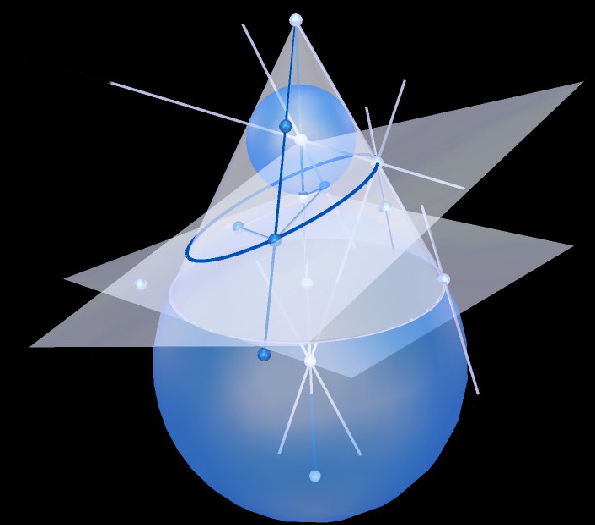
\includegraphics[width=0.7\textwidth]{figures/transparency}
	\caption{Erfolgreich dargestellte Transparenz}
	\label{fig:transparency}
\end{figure}


\begin{figure}[h]
%placing with [tb][h][t]
	\centering
	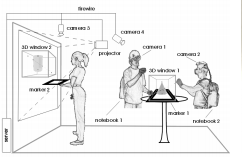
\includegraphics[width=1\textwidth]{figures/classroom}
	\caption{Augmented Classroom}
	\label{fig:samplefigure}
\end{figure}

%\subsection{Computergrafik know-how}
Entwickelt und forscht man an der Darstellung von virtuellen Objekten im Raum, so tun sich mitunter ungeahnte Schwierigkeiten auf, auf diese wird im Folgenden eingegangen.
\subsection{Statische und dynamische Geometrie}
Analysen aus den ersten Forschungsergebnissen haben gezeigt, dass es signifikant schwieriger ist, vorgegebene Koordinaten in virtueller Realität zu finden und Punkte zu manipulieren, als im zweidimensionalen Raum. Aufgrund von Tremor (natürliches Zittern der Hände) und mangels Hand-Auge-Koordination ist es schwierig, einen Punkt genau zu treffen \cite{1667626}. 
Wie mehrere Studien zeigen, bietet es sich in manchen Situation trotzdem an, auf eine zweidimensionale Darstellung zurückzukommen, da die 6 Freiheitsgrade in der Darstellung nicht immer von Vorteil sind \cite{Bowman:1999:ITC:930593}. 
Die exakte Eingabe von Koordinaten ist allerdings notwendige Voraussetzung, um mittels dynamischer Geometrie Software starre Körper drehbar zu machen. Es sollte schließlich auch möglich sein, mehrere Objekte miteinander zu verbinden um ``was-wäre-wenn-Szenarios'' ausprobieren zu können. Mit traditionellen Methoden ist es wesentlich wichtiger, die Position des Objekts im Raum darstellen zu können, dieser Aspekt verliert im dreidimensionalen Raum etwas an Signifikanz \cite{1667626}. 
\subsection{Nebenwirkungen - Simulator Sickness}
Ähnlich zu der schon bekannten Motion-Sickness \cite{motionsickness}, die manchmal bei Videospielen oder bei Reisen mit dem Auto, Zug oder Schiff auftritt, die zu Übelkeit und Schwindelgefühlen führen kann, da der Gleichgewichtssinn im Innenohr die Informationen, die die Augen liefern, nicht schnell genug verarbeiten kann, wird dieser gestört und so es kann auch beim Arbeiten mit Construct3D zu einer Art Motion-Sickness, die hier allerdings
Simulatur Sickness genannt wird, kommen.
\noindent \\
In der Evaluierung im Jahr 2003 wurde von einigen Lernenden über Simulator Sickness berichtet. 20 Minuten nach dem Beginn des Arbeitens in der virtuellen Umgebung tauchten Kopfschmerzen und Augenbelastungen bei einer Schülerin auf, trotzdem wollte sie damit weiterarbeiten. Nachträglich stellte sich heraus, dass die Zeiten für die kontinuierliche Arbeit mit einem HMD zu lang gewählt waren. Da negative Nebenwirkungen ein allgemeines potenzielles Problem bei der Arbeit mit HMDs darstellen und die subjektive Erfahrung derNutzer\_innen erheblich beeinflussen, sind sie für alle VR/AR-Anwendungen relevant, die diese Displays verwenden. Mögliche Gründe für diese Nebenwirkungen sind Akkomodationsprobleme, niedrige Bildfrequenz, Verzögerung oder schlechtsitzende Helme 
Folglich wurde in der dritten Studie im Jahr 2005 die Trainingsdauer pro Einheit auf maximal 45 Minuten reduziert, der Hartplastikhelm durch einen leichteren Fahrradhelm ersetzt und von den Teilnehmenden selbstbestimmte Ruhezeiten eingeführt. Trotzdem spürten 75,56\% der 47 Teilnehmenden eine moderate Müdigkeit oder Erschöpfung und 61,36\% berichteten von einer leichten Augenbelastung. Einige hatten Kopfschmerzen (37,78\%) und Schwindelgefühl (35,56\%).Im Allgemeinen berichteten die meisten Teilnehmenden jedoch, dass sie keine schwerwiegenden Probleme hatten. Die meisten dieser Symptome könnten mit der Verwendung eines HMD zusammenhängen In Übereinstimmung mit den Beobachtungen und anderen Studien wurde empfohlen, die HMD-Nutzungszeit auf 20-30 Minuten pro Einheit zu beschränken  Basierend auf der Erfahrung trägt die Bildqualität von HMDs, insbesondere die Verzögerung und Qualität der Tracking-Daten, am meisten zu den berichteten Effekten bei \cite{Kaufmann_summaryof}.

\subsection{Evaluierungsergebnisse}
Im Folgenden werden gesammelte Forschungsergebnisse aus dem Paper ``Summary of Usability Evaluations of an Educational Agumented Reality Application zusammengefasst: \\
In einer ersten Evaluierung mit 14 Lernenden war eindeutig zu sehen, dass es nicht notwendig ist, den Schülerinnen und Schülern die Handhabung zu erklären und dass die Bereitschaft eine Umgebung der erweiterten Realität zu benutzen, auch besteht. Es konnte beobachtet werden, dass alle Teilnehmenden aber stolz auf ihre Konstruktionen waren und freudig ihr Werk rundherum begutachteten. Die Hand-Auge-Koordination war in erster Instanz noch etwas schwierig für die Versuchspersonen und alle hatten Probleme damit, Punkte an vorgegebene Koordinaten richtig zu setzen, woraufhin zusätzlich ein Raster eingebaut wurde \cite{Kaufmann:2002:MGE:1242073.1242086}.
Aus den Evaluierungsergebnissen von 2003 lassen sich folgende Aspekte ableiten: \\
Von technischer Seite gibt es noch Probleme mit der Benutzerfreundlichkeit von Hard,- und Software. Die Orientierung zwischen Benutzenden und konstruiertem Objekt muss verbessert werden. Weiters können noch Verbesserungen im Bereich des Wohlbefindends während der Verwendung und des kognitiven Verständnisses der Lernenden stattfinden.  Es lässt sich aber schon jetzt extrapolieren, dass ein messbarer Lernfortschritt mit der neuen Technologie erzielbar ist. \cite{article}. \\
Im Jahr 2003 wurde eine Studie auf Basis von Interviews und dem standardisierten Usability-Fragebogen ISONORM 9241/10 durchgeführt \cite{Kaufmann_summaryof}. Eine Reihe von Trainingsübungen wurde entwickelt, die zum österreichischen deskriptiven Geometrie-Curriculum der 11. und 12. Klasse passen \cite{Kaufmann_summaryof}.  Daran arbeiteten die Teilnehmenden (9 Schüler, 6 Schülerinnen) mit Hilfe ihrer Lehrenden. Jede Person nahm an 5 Trainingseinheiten mit einer Dauer von insgesamt 6 Stunden teil. Die Bewertung danach zeigte, dass die von Lernenden hoch bewerteten Kategorien (siehe Abb. \label{stat1}) auch den subjektiv gesehenen höchsten Prioritäten einer Bildungsanwendung (einfach bedienbar, schnell erlernbar; ermutigend, neues auszuprobieren; konsistent und im Gedächtnis bleibend) entsprechen \cite{Kaufmann_summaryof}.\\
Qualitative Forschung im Jahr 2006 hat ergeben, dass sowohl die ``Eignung zum Lernen'', als auch die ``Eignung zur Umsetzung der Aufgabe'' mit dem vorgegebenen Setting für die Testpersonen zur vollsten Zufriedenheit ausgefallen ist, was besonders wichtig für dieses Projekt ist. Auch insgesamt hat die Umfrage ergeben, dass die Benutzer\_innen mit den Möglichkeiten, sowie mit der Handhabung und der konsistenten Benutzungsmöglichkeit sehr zufrieden waren \cite{1667626}.
\noindent \\
\begin{figure}[t]
%placing with [tb][h][t]
	\centering
	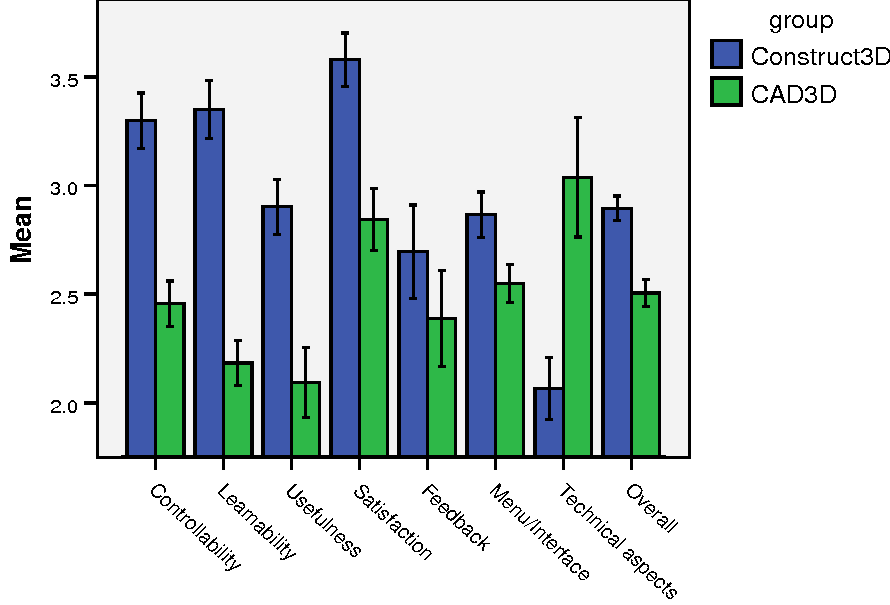
\includegraphics[width=0.9\textwidth]{figures/stat1}
	\caption{Usability Bewertungen von Lernenden}
	\label{fig:stat1}
\end{figure}
\begin{figure}[t]
%placing with [tb][h][t]
	\centering
	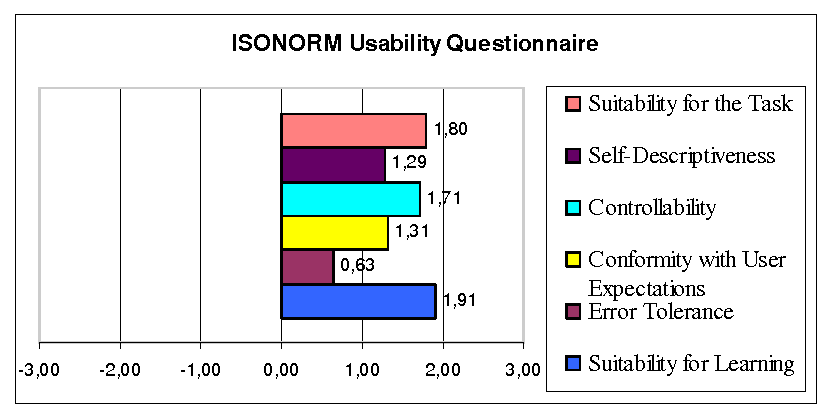
\includegraphics[width=0.9\textwidth]{figures/isonorm}
	\caption{Statistik über Symptome während der Benutzung}
	\label{fig:isonorm}
\end{figure}
Es wurden bessere Beschriftungen zu Construct3D hinzugefügt, sowie eine Hilfe-Box auf dem Panel, um alle Menüelemente zu erklären. Neben der neuen Strukturierung des Menüsystems wurde auch das visuelle Design von geometrischen Objekten verbessert  \cite{Kaufmann_summaryof}.  Eingeführt wurden Transparenz-Verwendung, konsistente Farbcodierung, Ebene-Trennung und automatische Vorschau neuer Objekte  \cite{Kaufmann_summaryof}. Nähere Informationen zu den Verbesserungen siehe \textit{Designing Immersive Virtual Reality for Geometry Education.}\\
Die dritte Auswertung war im Jahr 2005  \cite{Kaufmann_summaryof}. Verglichen wurde das Lösen von geometrischen Problemen mit Construct3D mit einer pädagogischen Desktop-Anwendung namens CAD3D. Teilnehmenden waren österreichische Oberstufenschüler\_innen im Alter zwischen 16 und 19 Jahren (M = 17,49, SD = .79; 44 (48,4\%) männlich und 47 (51,6\%) weiblich) \cite{Kaufmann_summaryof}. Sie nahmen an 6 Trainingseinheiten teil, die 45 Minuten dauerten [4, S.665]. In beiden Gruppen betreute ein Tutor oder eine Tutorin zwei Lernenden beim Arbeiten an den Geometrieaufgaben  \cite{Kaufmann_summaryof}.. Zur Beurteilung der Benutzerfreundlichkeit wurden Fragenbogen entwickelt, die von 8 etablierten Usability-Fragebögen angepasst waren (7 Skalen (siehe Abb. \label{stat1}  insgesamt 28 Fragen)  \cite{Kaufmann_summaryof}..
\noindent \\
Die Analyse der Fragenbogen ergab, dass Construct3D ein hochgradig benutzerfreundliches System ist, das - aus Usability-Sicht - mehrere Vorteile gegenüber der traditionellen Desktop-basierten Anwendung aufweist \cite{Kaufmann_summaryof}. Die niedrigen Bewertungen für technische Aspekte deuten jedoch darauf hin, dass es noch Probleme bezüglich der technischen Robustheit gibt, die angegangen werden müssen \cite{Kaufmann_summaryof}. Seltene Systemabstürze und kleinere technische Probleme können die Motivation der Teilnehmer und die Benutzerfreundlichkeit des Systems beeinträchtigen. Construct3D sollte hauptsächlich für Lehrinhalte verwendet werden, die eine dynamische 3D-Geometrie verwenden oder die Visualisierung abstrakter Probleme erfordern \cite{Kaufmann_summaryof}. In Bezug auf die bevorzugte Trainingseinrichtung der Lernenden zwischen Construct3D und CAD3D gab es keine signifikanten Unterschiede. Die Mehrheit der Lernenden möchte Construct3D in der Schule einsetzen (ja = 64,44\%, eher ja = 26,67\%); 8,89\% möchten das System lieber nicht in der Schule einsetzen \cite{Kaufmann_summaryof}.  Die Kommentare zu den potenziellen Problemen beim Einsatz von Construct3D in Schulen betrafen vor allem fehlende Finanzierung und die Robustheit der Hardware und Software \cite{Kaufmann_summaryof}.\\

\section{Zusammenfassung}
Zusammenfassend lässt sich sagen, dass die Forschung auf dem Gebiet der virtuellen und erweiterten Realität für die Aus- und Weiterbildung signifikant ist, da der traditionelle Frontalunterricht eher nicht mehr zeitgemäß ist, da wir uns im sogenannten ``Expierence Age'' befinden. Diese Generation an Lernenden kommt bereits sehr früh mit neuen Medien als auch dem Internet in Kontakt und lernt anders als es noch frühere Generationen getan haben \cite{Hu-Au}. \\
Hannes Kaufmann hat mit seiner Forschung schon sehr früh einen wichtigen Beitrag zur Fortentwicklung von Lehrmethoden und der Entwicklung eines modernen Klassenzimmers beigetragen. 
Die Konzepte lassen sich auch auf Bereiche der Erwachsenenbildung und den Begriff ``Lifelong-learning'' anwenden. 

%\section{Literaturverweise}
\label{sec:bib}

\printbibliography

\end{document}
